\section{Implementation and Evaluation}\label{sec:implem_eval}

We have implemented \Slice{} as a compiler that transforms continuous probabilistic programs into either fully or partially discretized programs. Fully discretized programs are translated and analyzed using the discrete exact inference engines \Dice{} (2020)~\cite{Holtzen2020Dice} and \Roulette{}~\cite{Moy2025Roulette}. Figure~\ref{fig:architecture} on page \pageref{fig:architecture} shows the overall architecture of the \Slice{} system for fully discretized programs.
%In contrast, partially discretized programs can be analyzed using heterogeneous inference engines, which support combining multiple inference strategies such as exact and approximate methods within a single probabilistic program. Figure~\ref{fig:architecture} shows the overall architecture of the \Slice{} system for fully discretized programs.

The \Slice{} compiler consists of approximately 3,400 lines of OCaml code (including the lexer, parser, type inference and discretization engines, \Dice{}/\Roulette{} code generators, a sampling-based interpreter, and statistical equivalence checking). We use the OCaml GSL package~\cite{gsl} to compute the CDFs of the probability distributions. The system is open-source and available at \url{https://github.com/[anonymized]}, along with benchmarks, documentation, and a Docker image. All benchmarks were run within that Docker image on an Apple M3 with 16GB RAM.

%\medskip
%As we will see through several benchmarks, the performance of \Slice{} is competitive with existing state-of-the-art exact and approximate inference solvers for hybrid probabilistic programs. In particular, we evaluate \Slice{} using \Dice{} and \Roulette{} as backends against the exact inference solver SPPL~\cite{Saad2021SPPL} and the approximate inference solver HyBit~\cite{Garg2024BitBlast} on three sets of benchmarks. First, a series of synthetic benchmarks designed to test the how well \Slice{} scales asymptotically compared to SPPL. Second, a set of benchmarks for verifying fairness properties of decision trees. Lastly, we evaluate \Slice{} on a series of small baseline programs commonly used to test PPLs in the literature. 
%All experiments used Dice (2020) and Roulette (Racket 8.13, Rosette 4.1).

In what follows, we evaluate the performance of using \Slice{} with \Dice{}/\Roulette{} for exact inference on (i) a set of synthetic benchmarks and (ii) a set of benchmarks taken from the literature, comparing to the state-of-the-art tool SPPL for exact inference of continuous probabilistic programs.

\subsection{Evaluating \Slice{} on Synthetic Benchmarks}\label{sec:synthetic-benchmarks}
We designed a set of synthetic benchmarks consisting of programs that can be scaled up in size, with varying dependencies between the program variables. Schematically:
%
    \begin{lstlisting}[aboveskip=0.1em,belowskip=.1em]
        let x1 = uniform(0,1) in 
        let x2 = if x1 < r1 then uniform(0,2) else uniform(0,3) in 
        let x3 = if x2 < r2 ...
        ...
        x_n < 0.5
    \end{lstlisting}
%
 Each program consists of a sequence of nested conditionals, where each branch depends on a previous variable sampled from a uniform distribution, proceeding until the final condition $x_n < 0.5$ is reached. Here $0 \leq r_i \leq 1$ are fixed float constants. With these programs, provided in in Appendix \ref{appen:synthetic-sketches}, we evaluate how \Slice{} scales for deep conditional branching and stochastic control flow. 
 
The programs in \Cref{fig:cond-benchmarks-a} follow the scheme depicted above where the program size is $n$, i.e., the number of comparisons performed is $n$. In \Cref{fig:cond-benchmarks-b}, each $x_i$ does not necessarily depend on $x_{i-1}$ but on some randomly chosen predecessor\footnote{We generate these programs in a randomized manner with a fixed seed for reproducability}. In \Cref{fig:cond-benchmarks-c}, we additionally choose at random whether the guards of the conditionals and the branches are either some predecessor variable $x_i$ or a  $\uniform$-sampling instruction.
 %\begin{figure}[h]
    \centering
    \begin{lstlisting}
        let x1 = unif() in 
        let x2 = if x1 < r1 then unif() else unif() in 
        let x3 = if x2 < r2 ...
        ...
        x_n < 0.5
    \end{lstlisting}
    \caption{Structure of synthetic programs used in our evaluation. Each program consists of a sequence of nested \texttt{if} statements, where each branch conditions on a previous variable sampled from a uniform distribution, proceeding until the final condition $x_n < 0.5$ is reached. $0 \leq r_i \leq 1$ is a random float. This construction allows us to test how well \Slice{} handles deep conditional branching and stochastic control flow.}
    \label{fig:nested-conditionals}
    \end{figure}

%\subsubsection{Conditional Independence}
%We test programs where each variable's distribution depends on comparisons with previous variables:
%
%\begin{itemize}
%\item Each variable $x_i$ depends on its immediate predecessor via a conditional branch $x_{i-1} < r_{i-1}$, forming a sequential dependency chain. See Figure~\ref{fig:cond-benchmarks-a}.
%\item Each variable $x_i$ depends on a randomly selected predecessor $x_j$ (for $j < i$) via a conditional branch $x_j < r_{i-1}$. See Figures~\ref{fig:cond-benchmarks-b}.
%\item Each variable $x_i$ uses a randomized conditional expression, where the guard and both branches may involve either a randomly selected predecessor $x_j$ (for $j < i$) or a freshly sampled uniform value. See Figure~\ref{fig:cond-benchmarks-c}.
%\end{itemize}
%
%
\begin{figure}[!t]
\centering
\begin{subfigure}{0.4\textwidth}
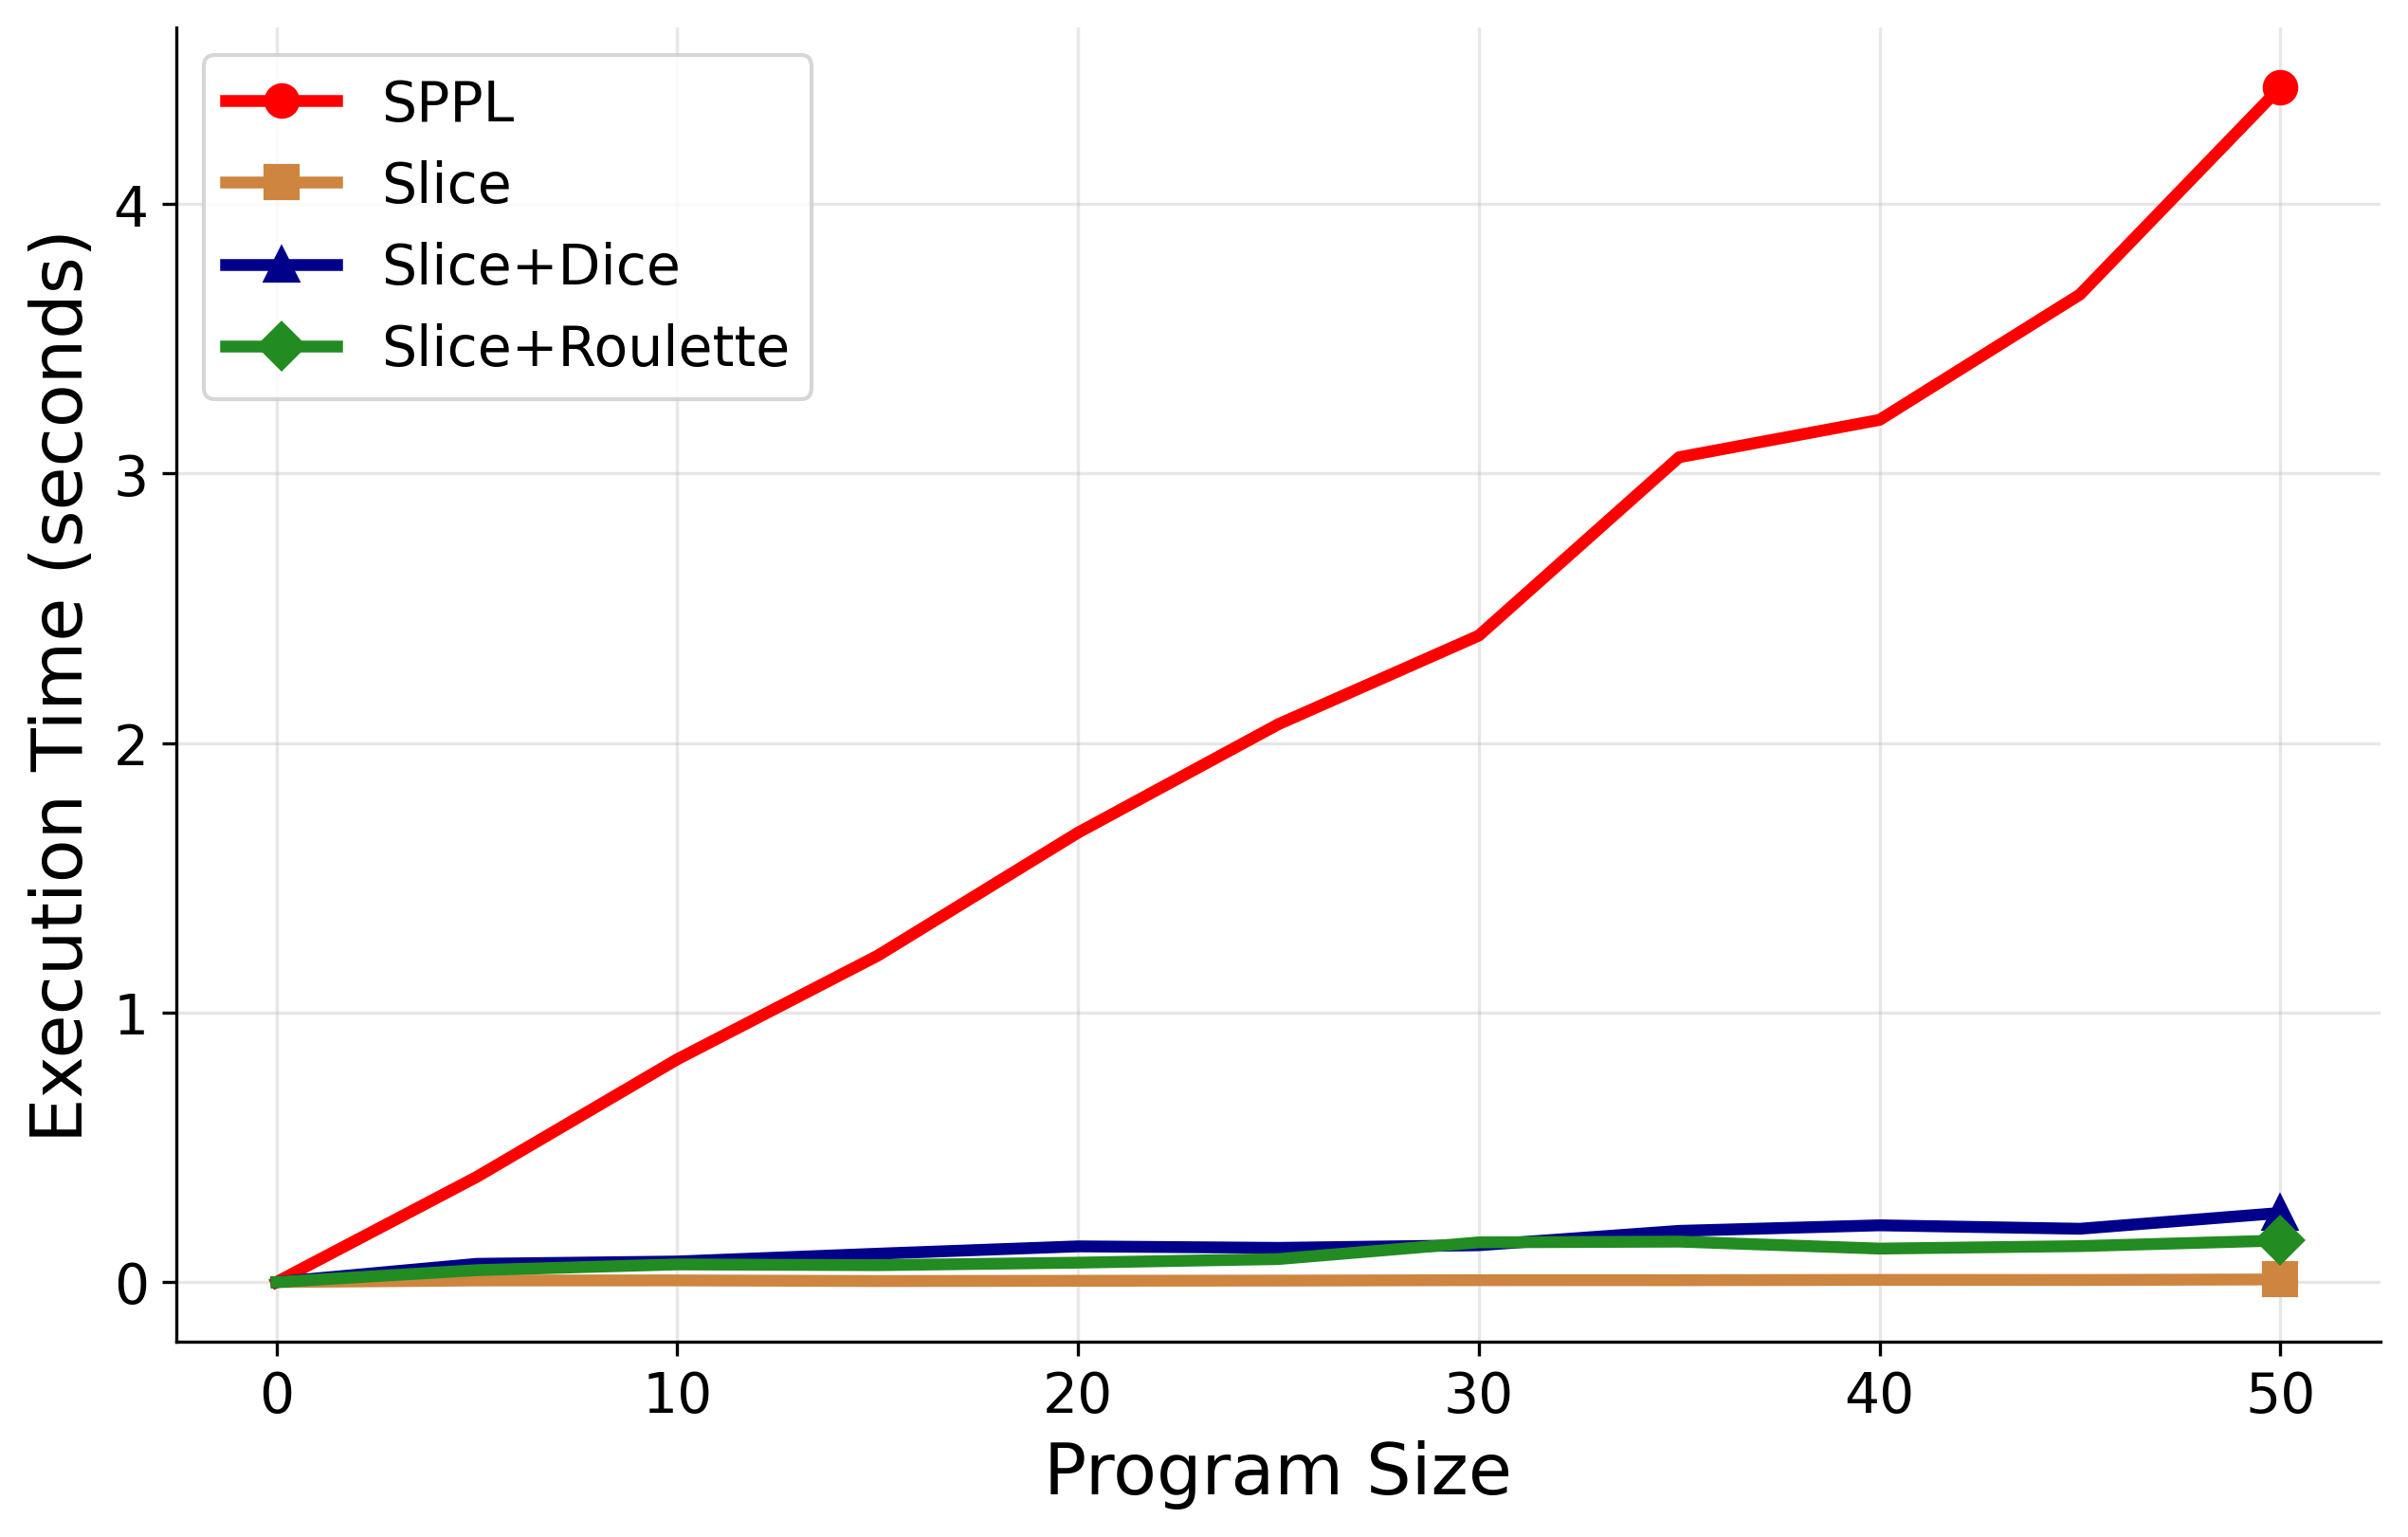
\includegraphics[width=\textwidth]{../images/scaling/build_conditional_independent_slice.png}
\caption{Conditional Independent}
\label{fig:cond-benchmarks-a}
\end{subfigure}
\hfill
\begin{subfigure}{0.4\textwidth}
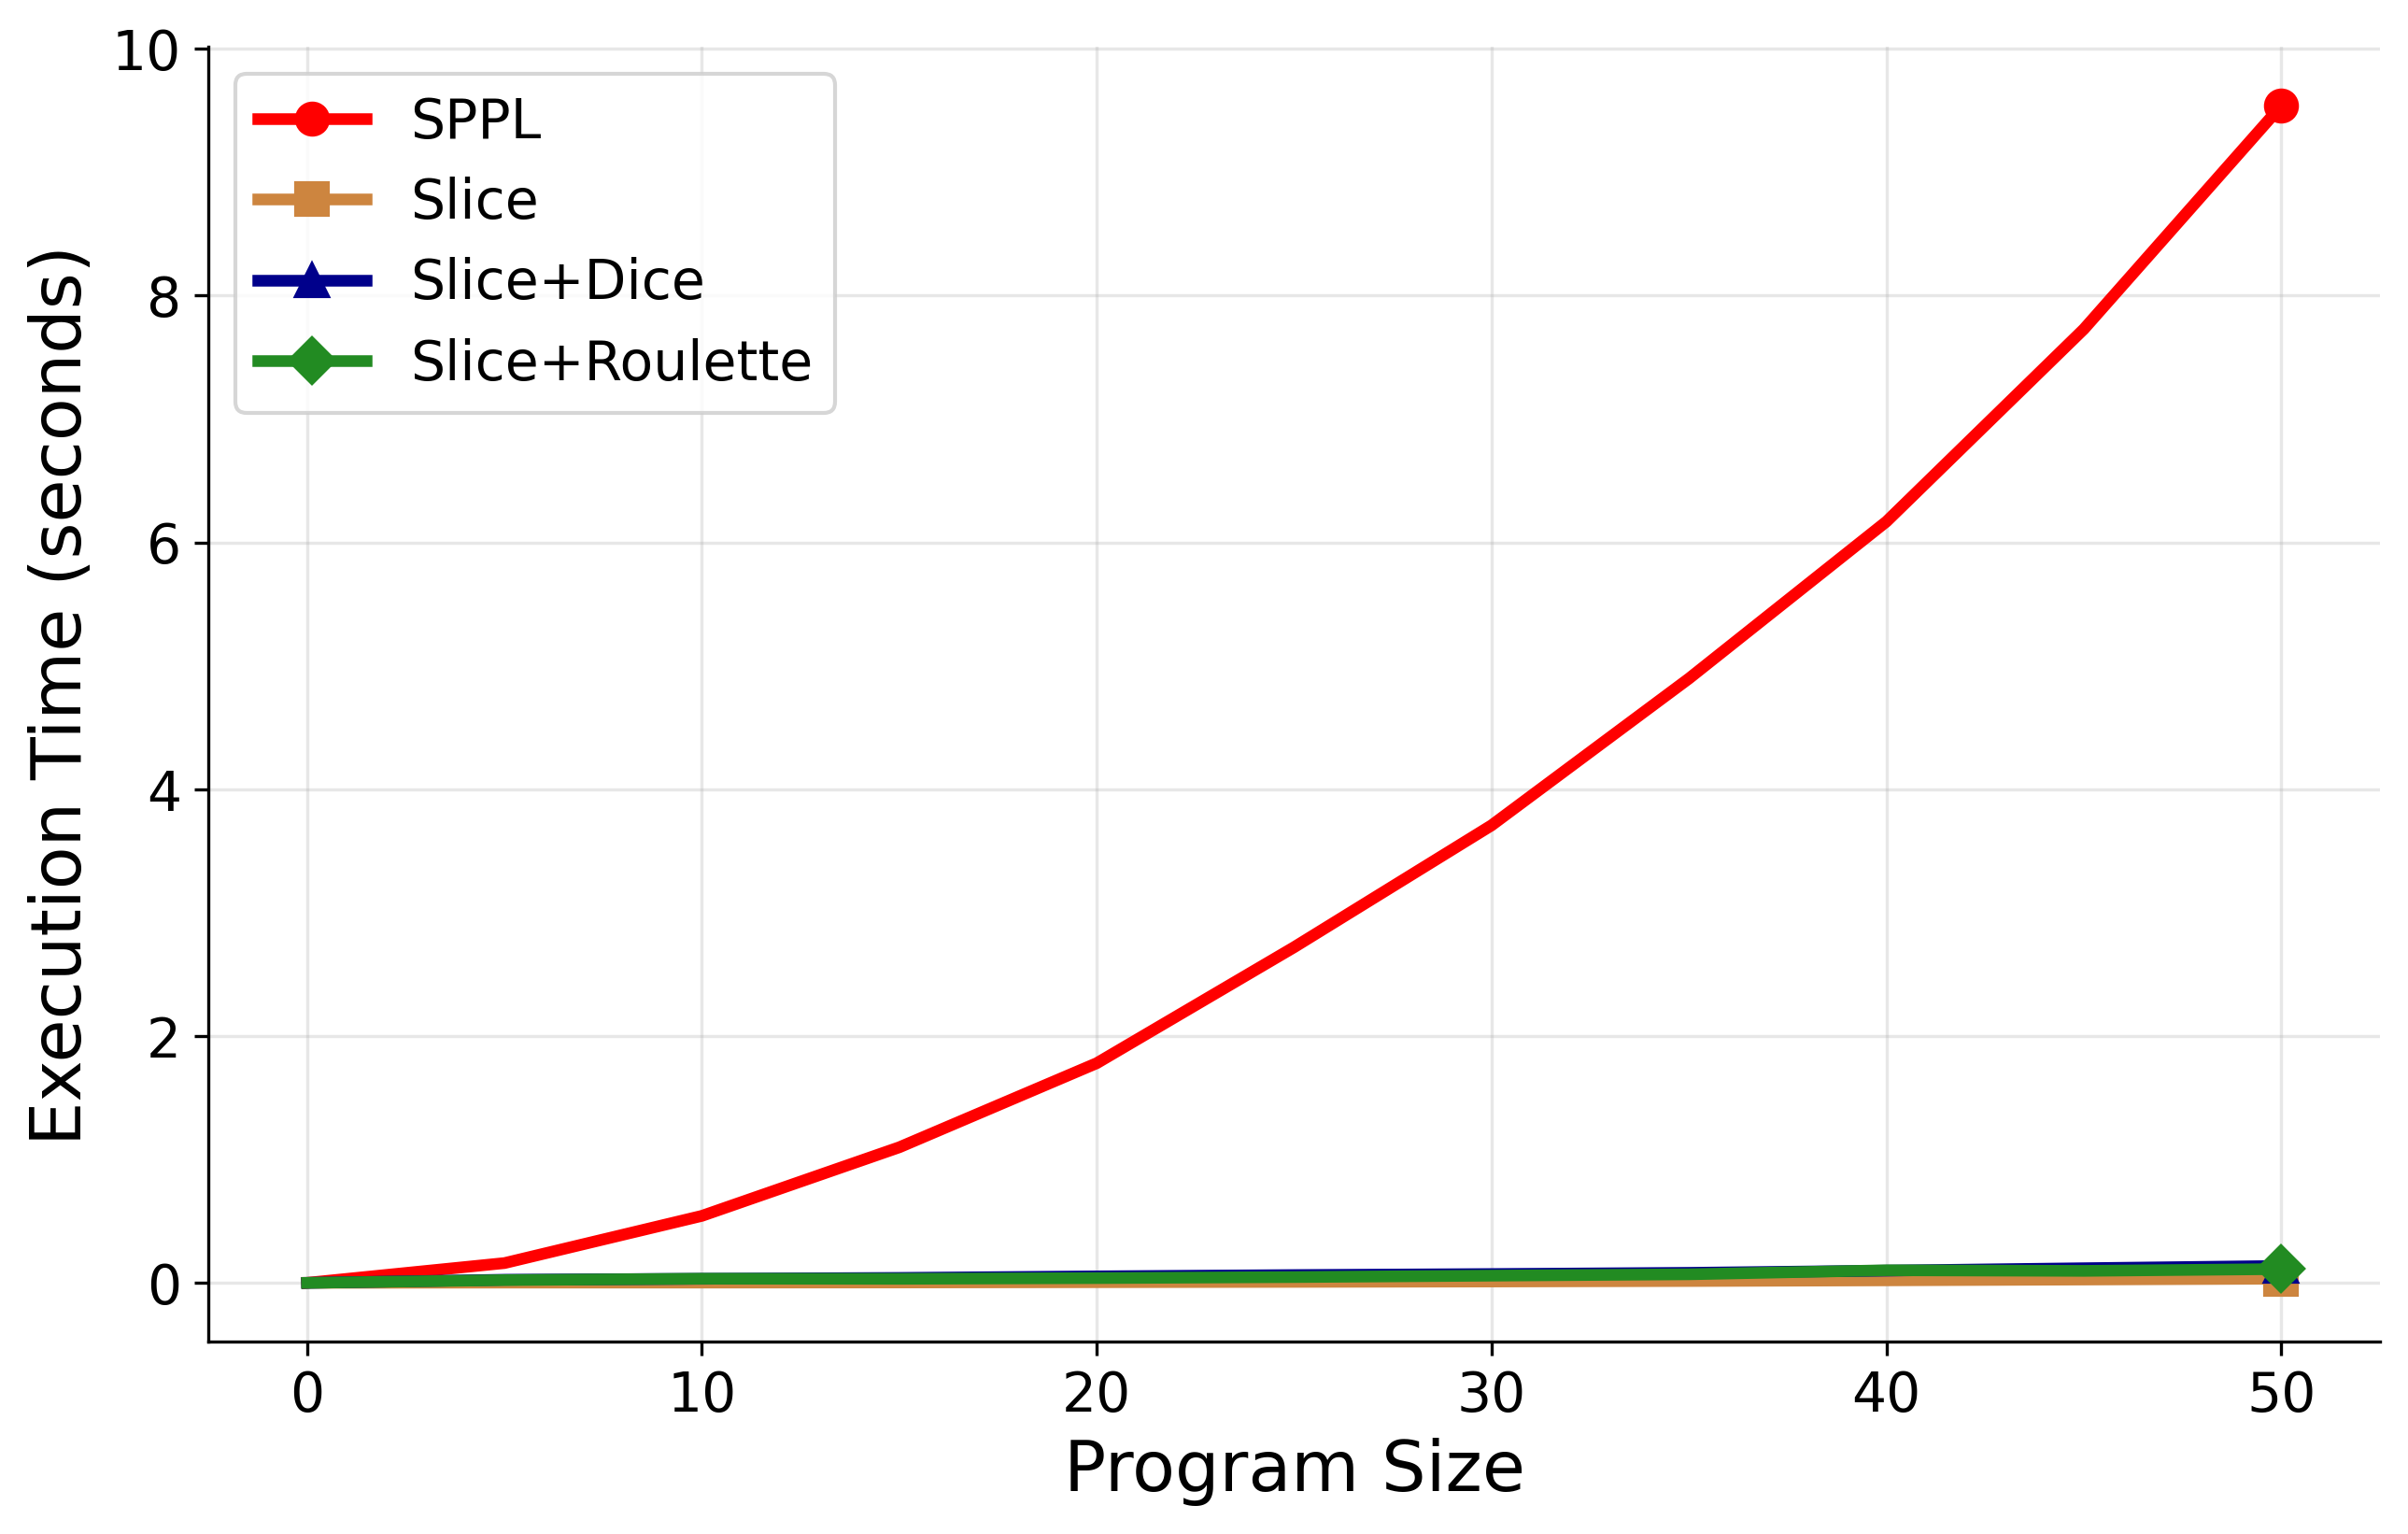
\includegraphics[width=\textwidth]{../images/scaling/build_conditional_independent_fork_slice.png}
\caption{Conditional Independent -- Fork}
\label{fig:cond-benchmarks-b}
\end{subfigure}
\hfill
\begin{subfigure}{0.4\textwidth}
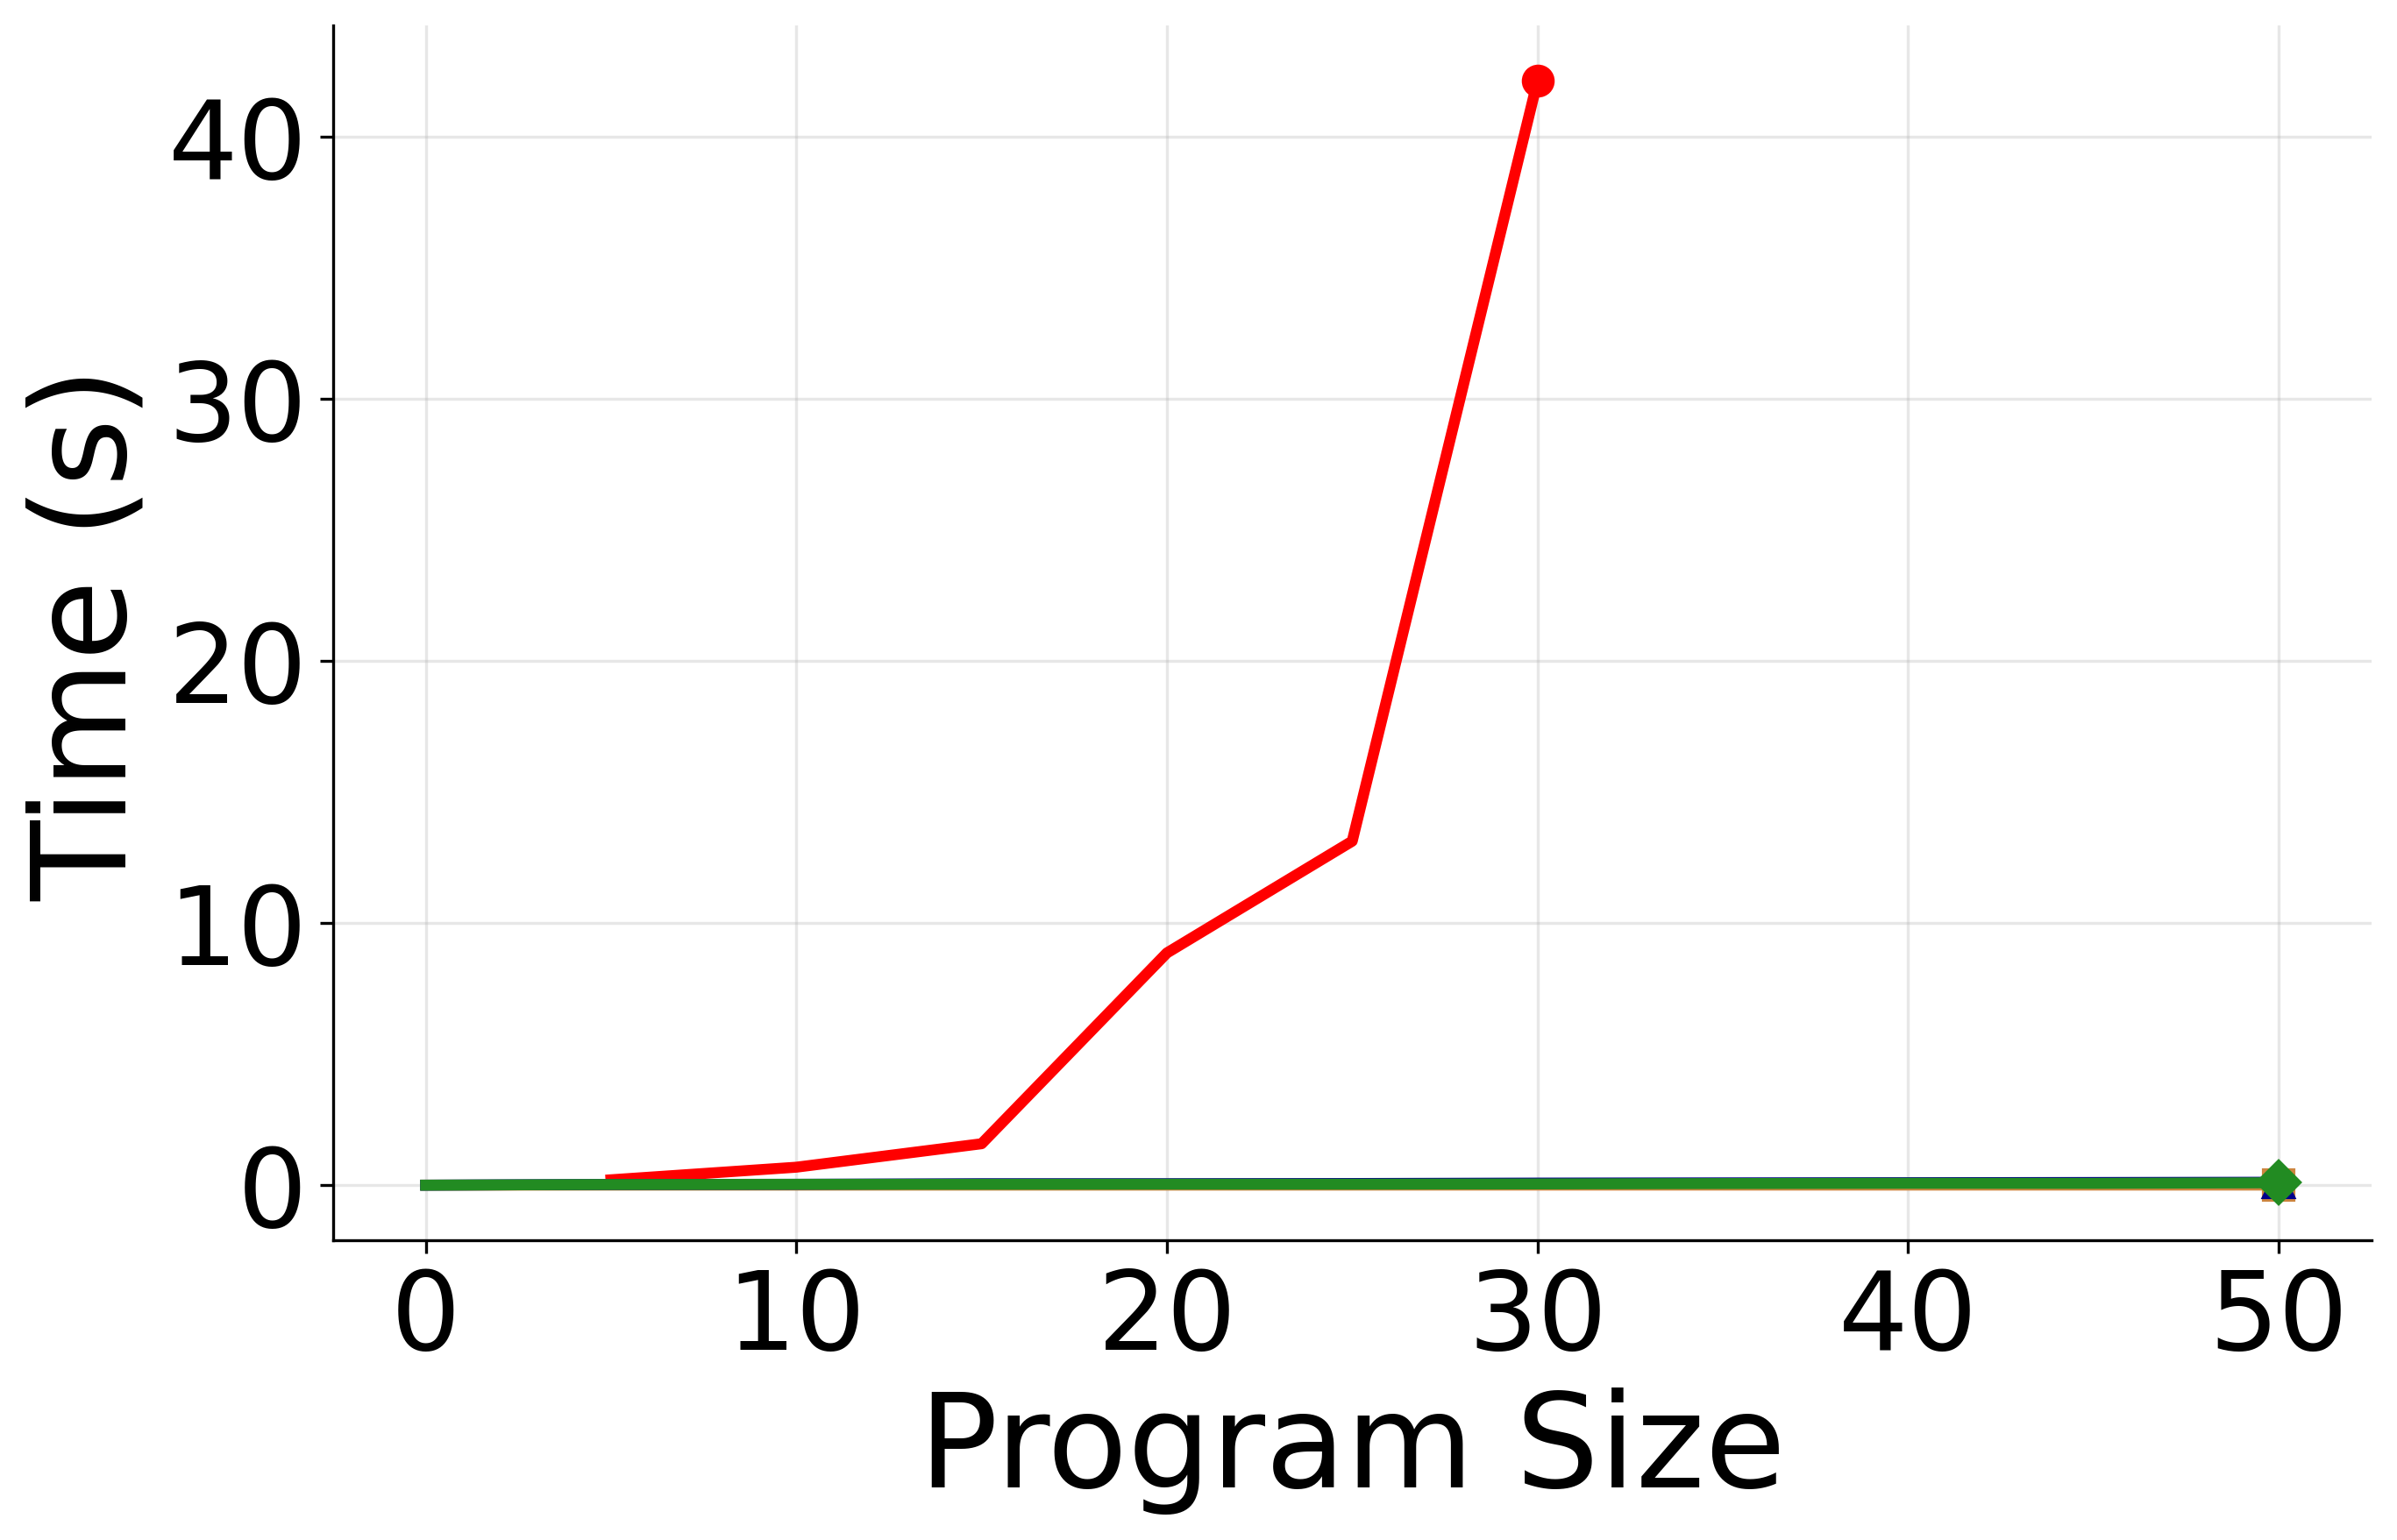
\includegraphics[width=\textwidth]{../images/scaling/build_conditional_random_independent_slice_1.png}
\caption{Conditional Independent -- Rand. 1}
\label{fig:cond-benchmarks-c}
\end{subfigure}
\hfill
\begin{subfigure}{0.4\textwidth}
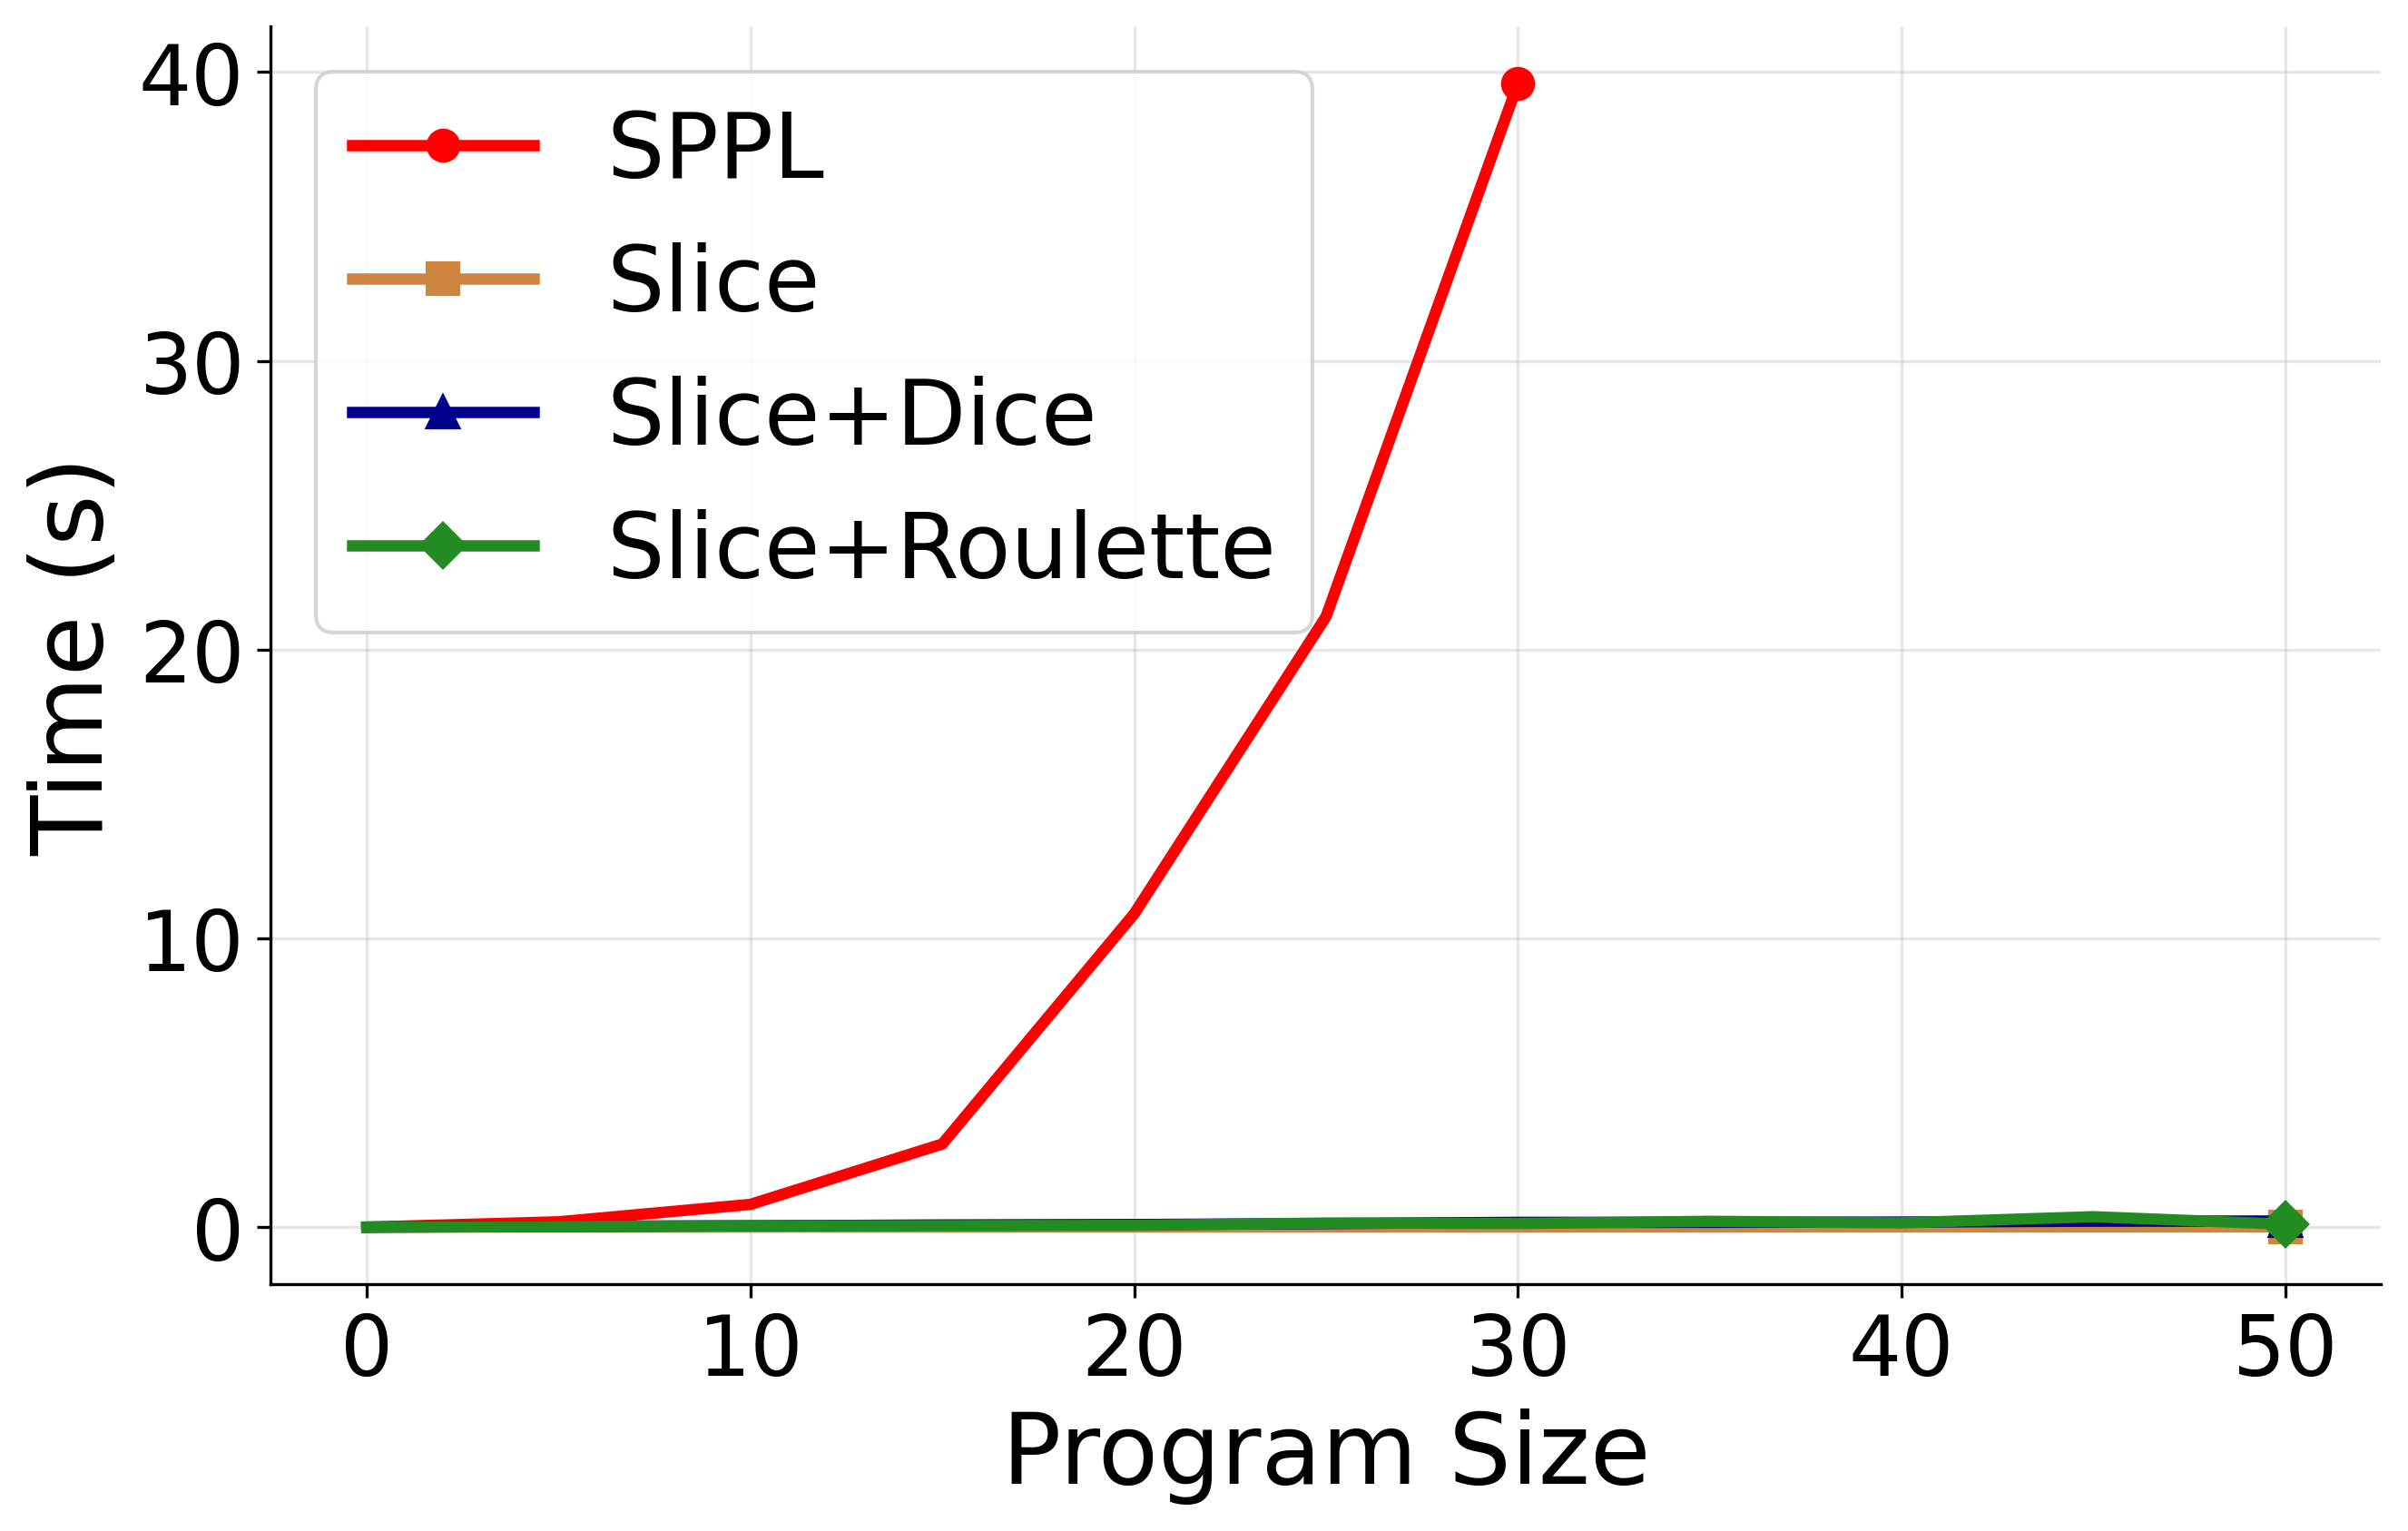
\includegraphics[width=\textwidth]{../images/scaling/build_conditional_random_independent_slice_2.png}
\caption{Conditional Independent -- Rand. 2}
\label{fig:cond-benchmarks-d}
\end{subfigure}
\caption{Scaling graphs for conditionally independent programs. Time-out=120s; a disappearing line indicates timeout. Graphs (a)--(d) correspond, respectively, to the representative programs in \Cref{fig:cond-benchmarks-a-example,fig:cond-benchmarks-b-example,fig:cond-benchmarks-c-example,fig:cond-benchmarks-d-example}.}
\label{fig:cond-benchmarks}
\end{figure}

%
 The programs in \Cref{fig:alt-benchmarks-a} also follow the scheme depicted above but where the variables used in the guards cycle with a fixed span size of $m$. For instance, for $m=2$, the pattern is $x_1,x_2,x_1,\ldots$. The programs in \Cref{fig:alt-benchmarks-b,fig:alt-benchmarks-c,fig:alt-benchmarks-d} follow a similar pattern, see Appendix~\ref{appen:synthetic-sketches} for details.

We depict the runtime (in seconds) of (i) SPPL (ii) \Slice{} (discretization only) (iii) \Slice{}+\Dice{} (discretization and subsequent inference using \Dice{}), and (iv) \Slice{}+\Roulette{} (discretization and subsequent inference using \Roulette{}). The time-out is 300 seconds.

%\subsubsection{Alternating Guards}
%We test programs in which comparison guards alternate in a pattern:
%
%\begin{itemize}
%\item Guard variables cycle with a fixed span. For example, with span 2, guards alternate as $x_1,x_2,x_1,\ldots$. See Figure~\ref{fig:alt-benchmarks-a}. Figures~\ref{fig:alt-benchmarks-b} and~\ref{fig:alt-benchmarks-c} show variants where the if and else branches are replaced with an immediate predecessor variable $x_{i-1}$ instead of a uniform distribution.
%
%\item Guard variables are selected based on a randomly chosen span at each step, rather than cycling deterministically as before. See Figure~\ref{fig:alt-benchmarks-d}.
%\end{itemize}

\begin{figure}[!t]
\centering
\begin{subfigure}{0.4\textwidth}
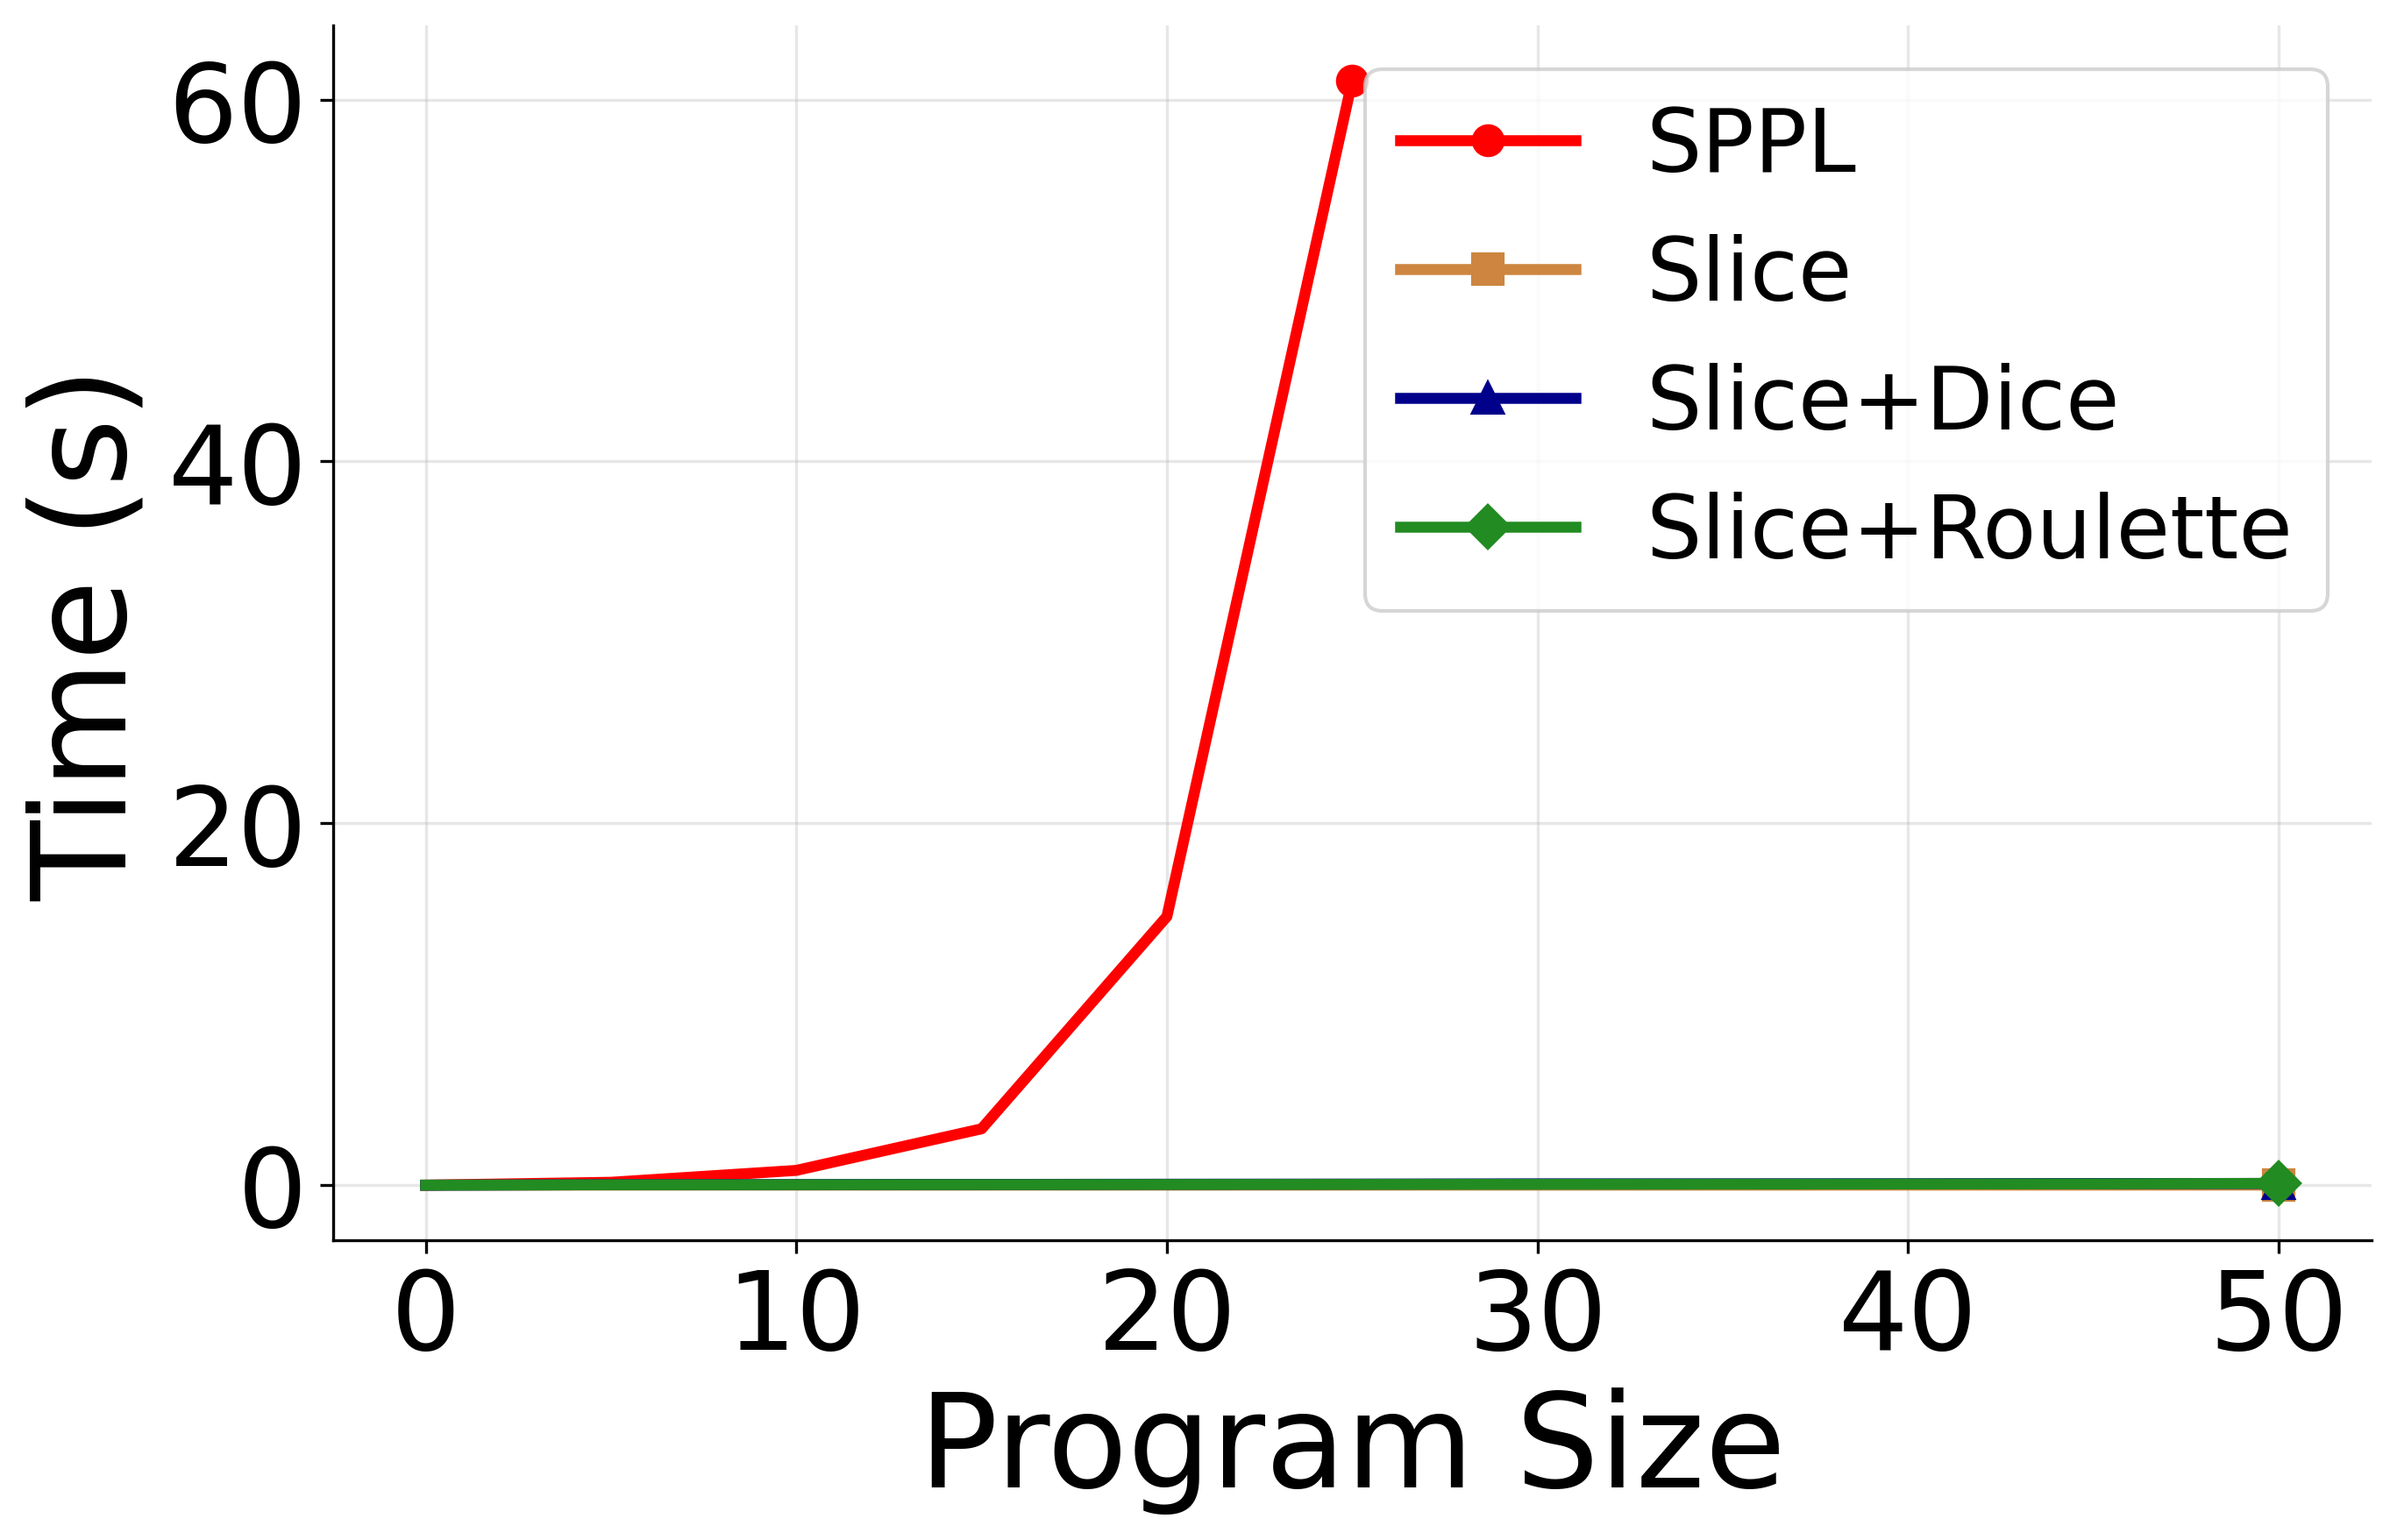
\includegraphics[width=\textwidth]{../images/scaling/build_alternating_guard_slice_1.png}
\caption{Alt. Guard 1}
\label{fig:alt-benchmarks-a}
\end{subfigure}
\hfill
\begin{subfigure}{0.4\textwidth}
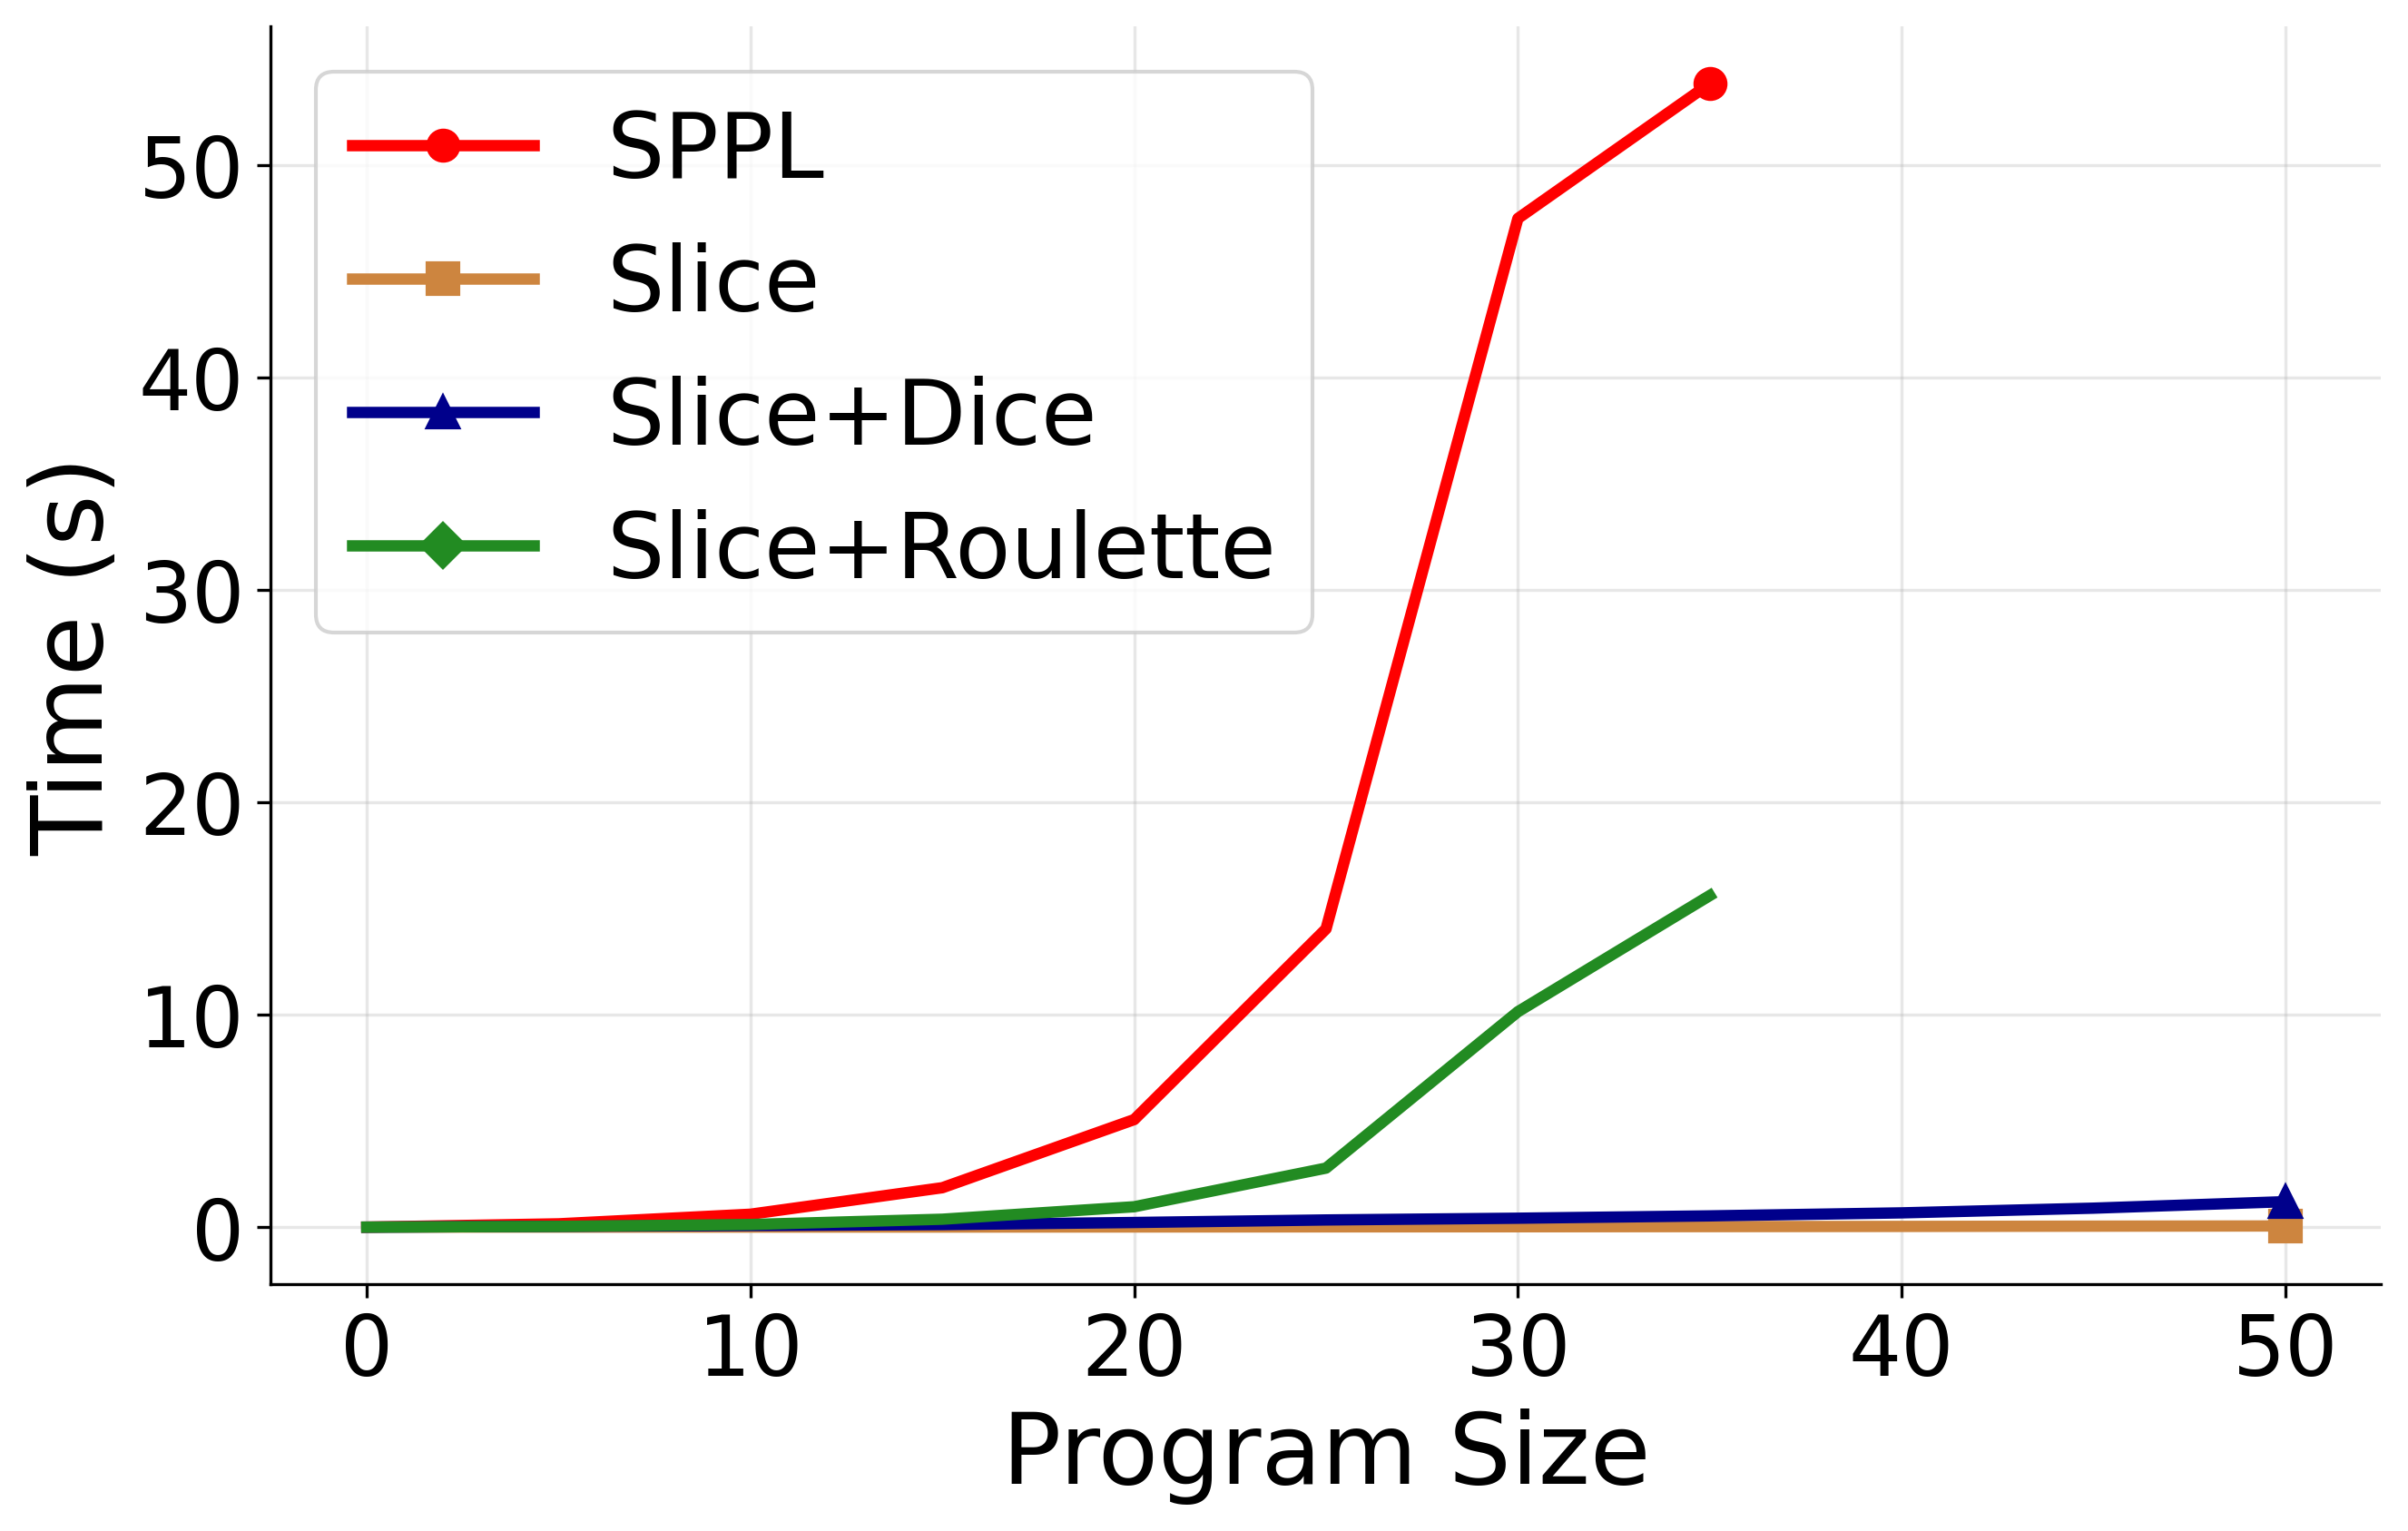
\includegraphics[width=\textwidth]{../images/scaling/build_alternating_guard_slice_2.png}
\caption{Alt. Guard 2}
\label{fig:alt-benchmarks-b}
\end{subfigure}
\hfill
\vspace{0.5em}
\begin{subfigure}{0.4\textwidth}
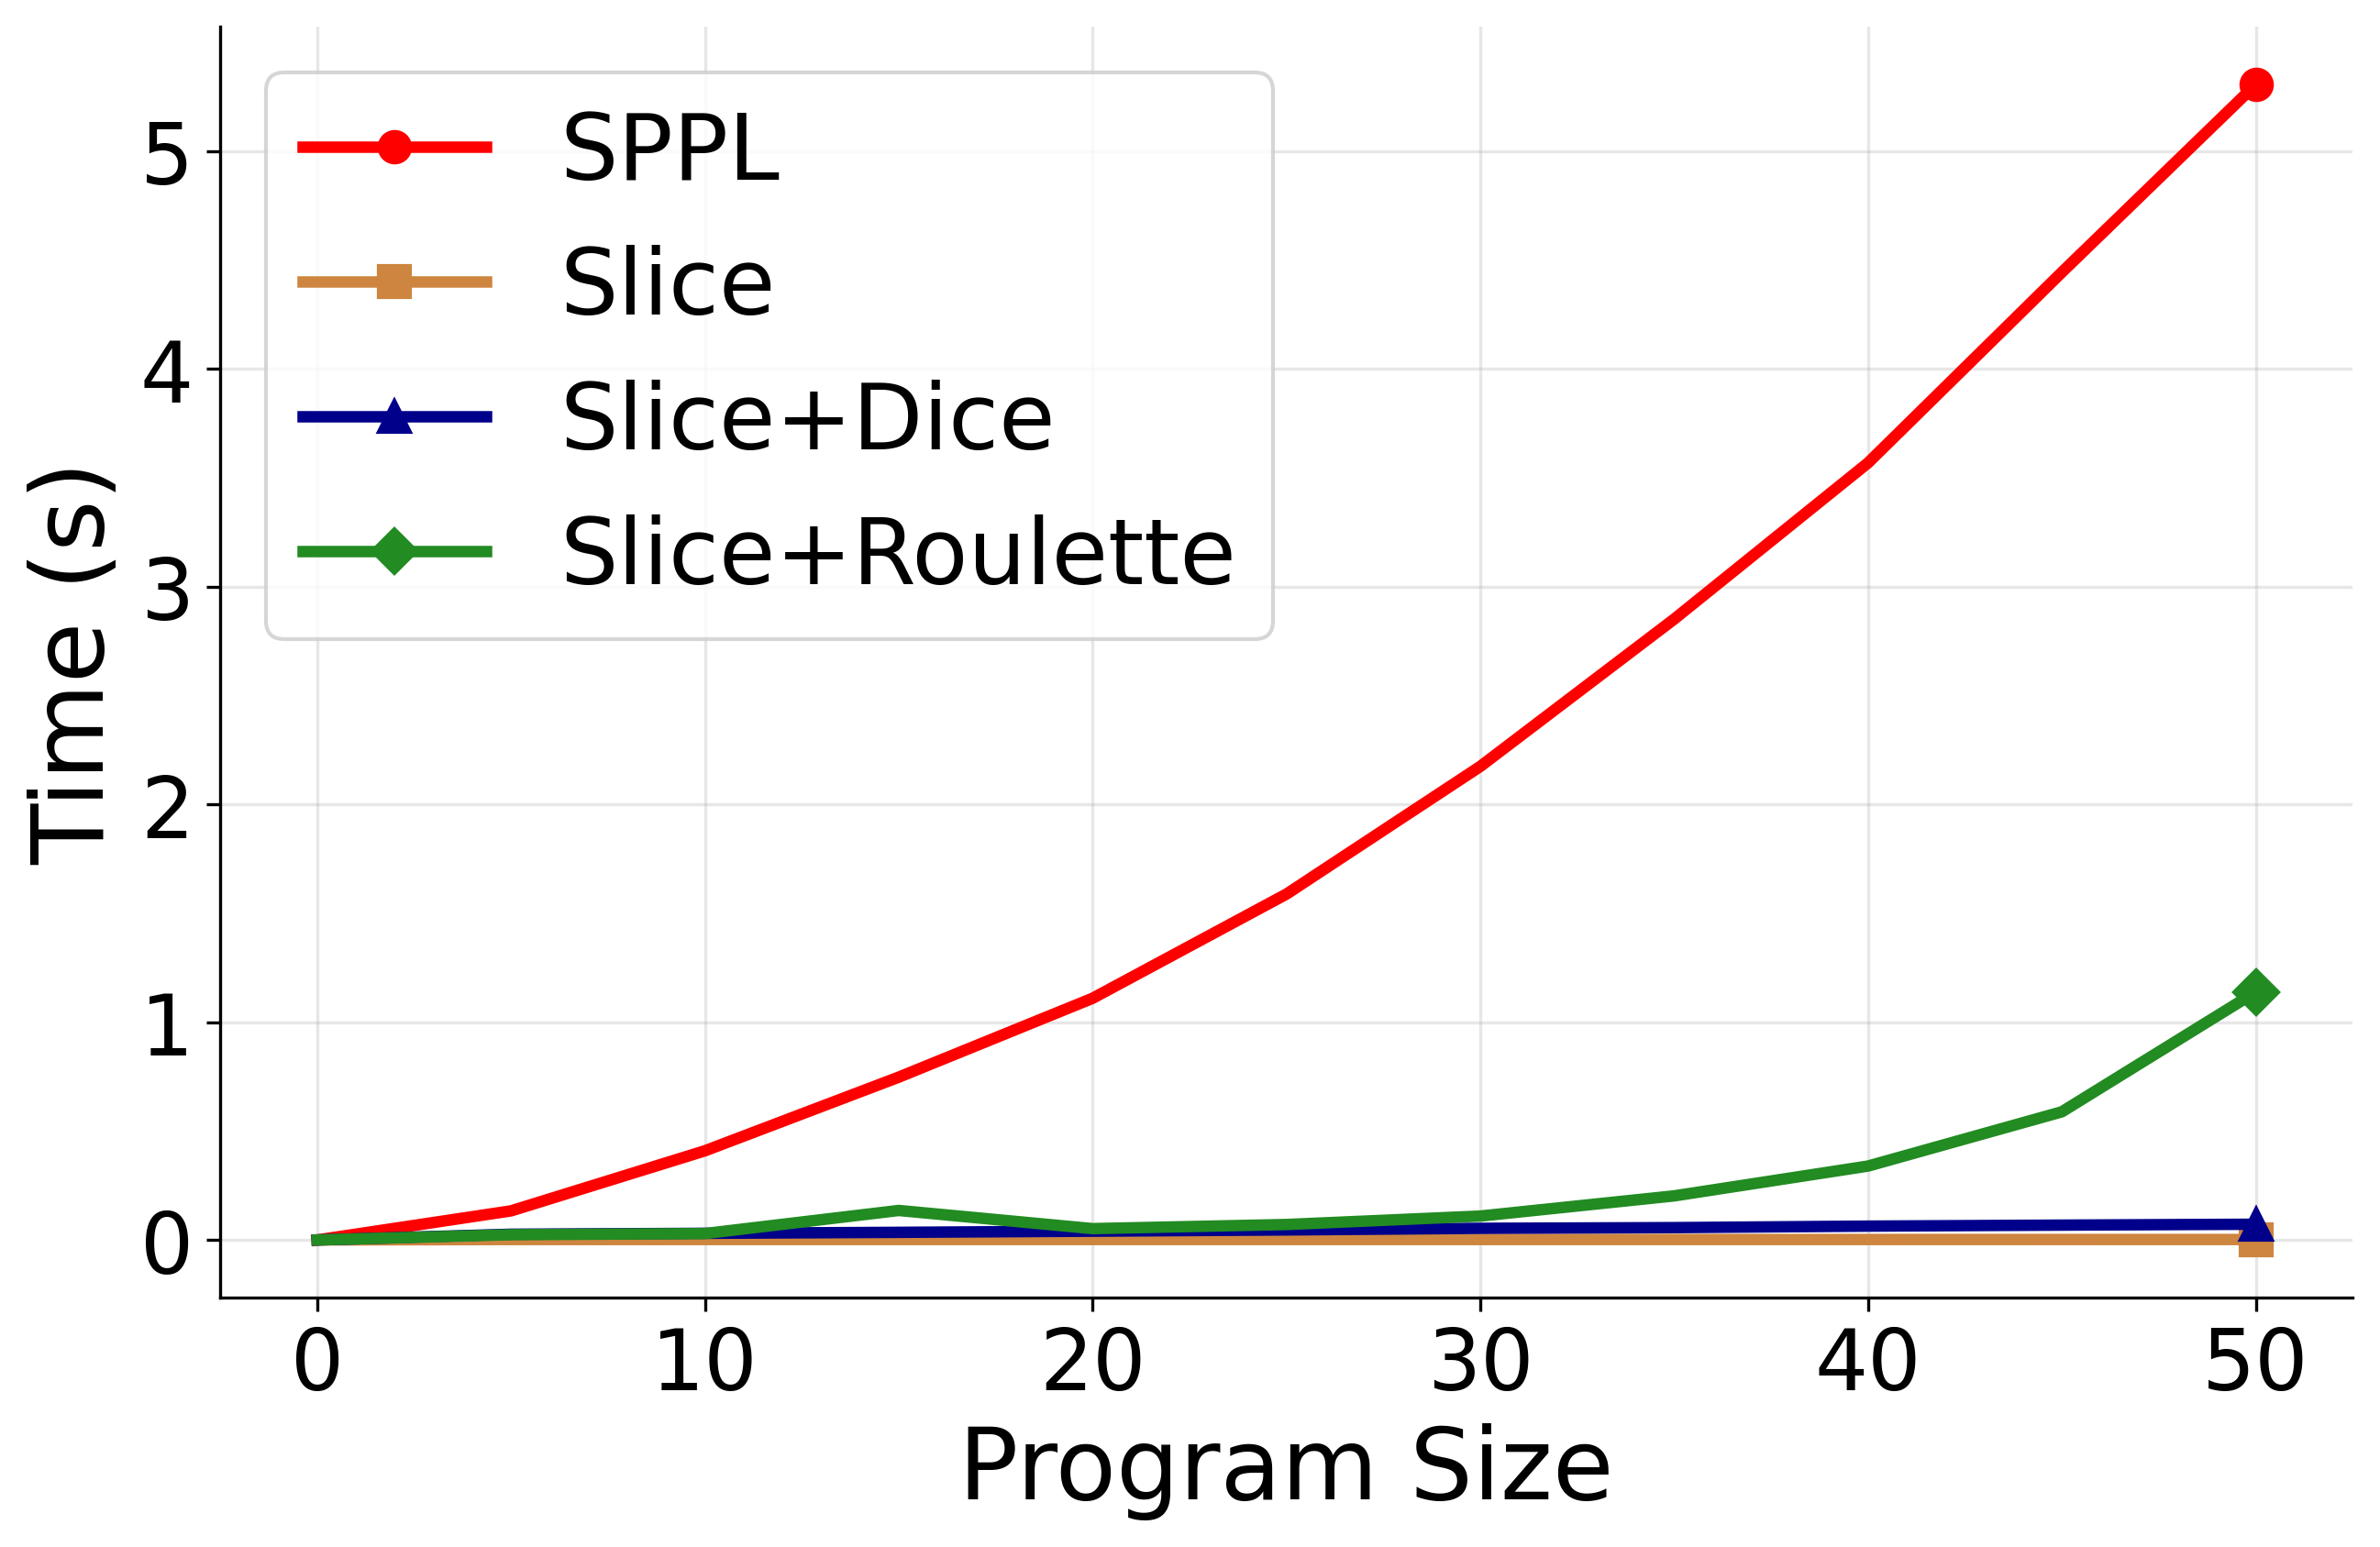
\includegraphics[width=\textwidth]{../images/scaling/build_alternating_guard_slice_3.png}
\caption{Alt. Guard 3}
\label{fig:alt-benchmarks-c}
\end{subfigure}
\hfill
\begin{subfigure}{0.4\textwidth}
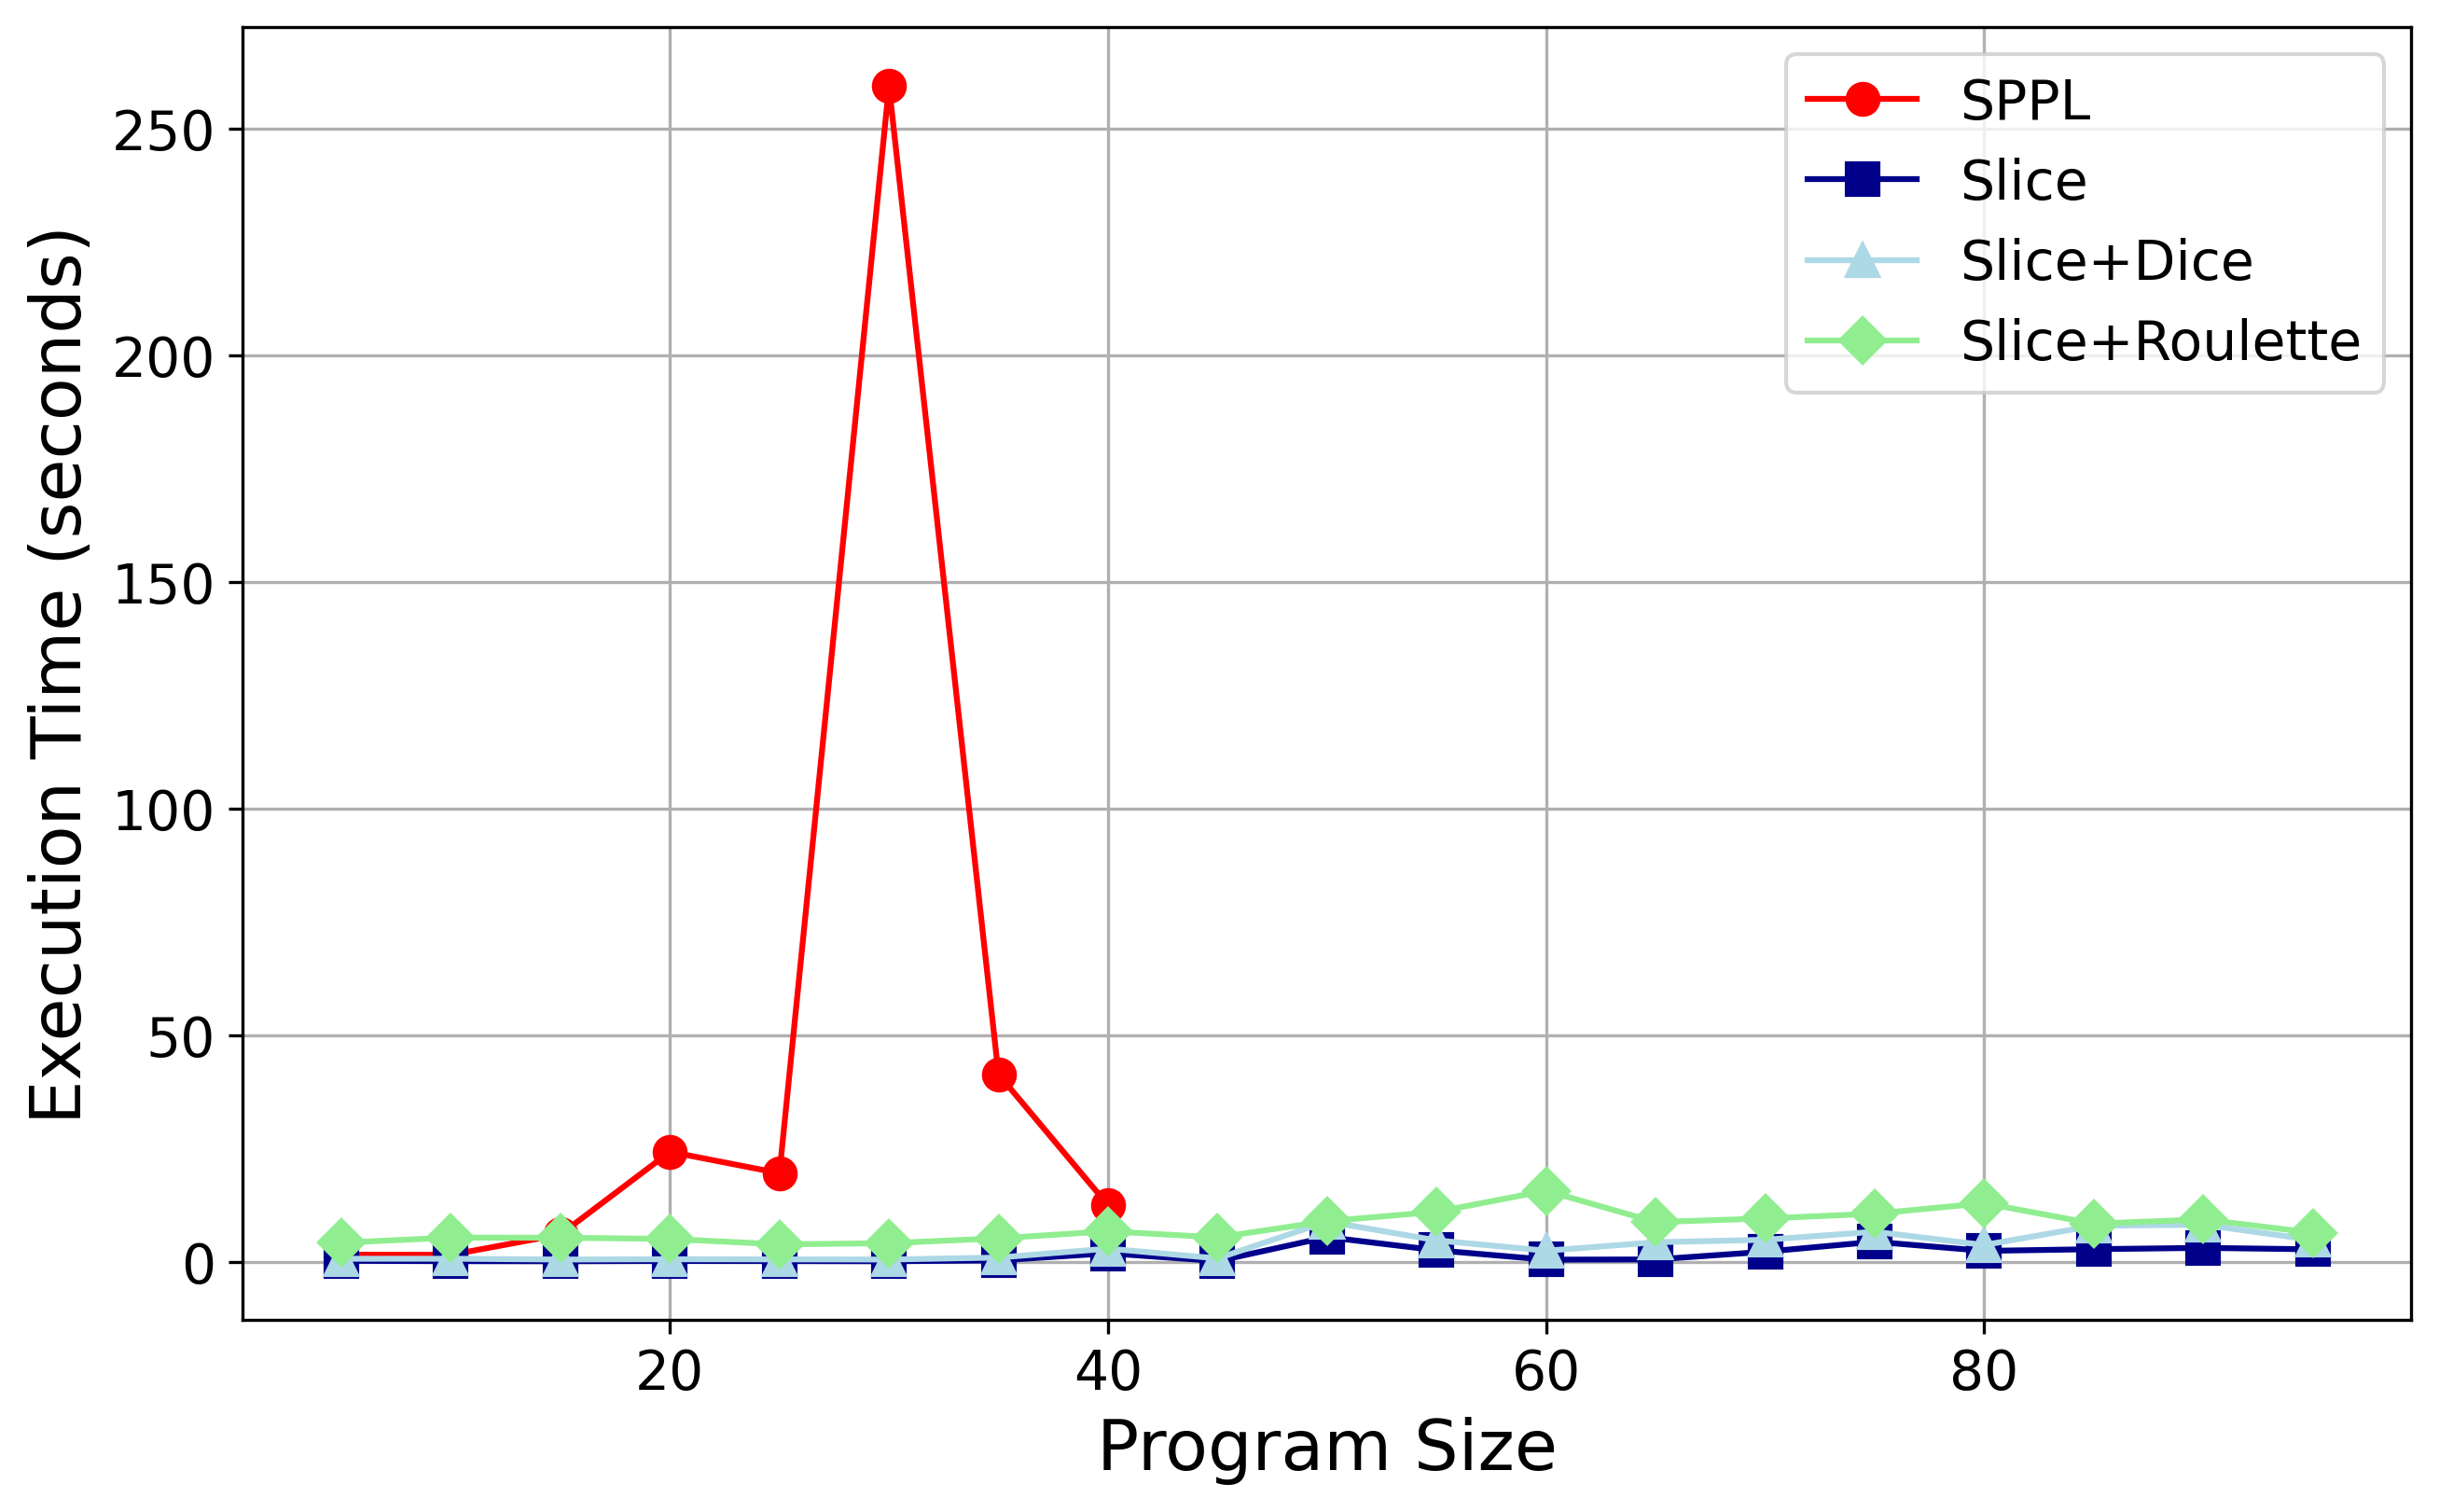
\includegraphics[width=\textwidth]{../images/scaling/build_random_alternating_guard_slice.png}
\caption{Alt. Guard -- Rand.}
\label{fig:alt-benchmarks-d}
\end{subfigure}
\caption{Results for alternating guard benchmarks. Time-out=120s. A disappearing line indicates a time-out.}
\label{fig:alt-benchmarks}
\vspace{-.2cm}
\end{figure}

\paragraph{Results.} The results indicate that exact inference with \Slice{} + \Dice{}/\Roulette{} can scale to large programs, often outperforming the state-of-the-art tool SPPL significantly. This is particularly striking in \Cref{fig:cond-benchmarks-b} and \Cref{fig:alt-benchmarks-a,fig:alt-benchmarks-b,fig:alt-benchmarks-d}, where the time required by \Slice{} + \Dice{}/\Roulette{}  remains roughly constant but increases rapidly for SPPL when increasing the program size. In \Cref{fig:cond-benchmarks-c}, we observe a mixed picture for programs of sizes $1-20$, with \Slice{} + \Dice{}/\Roulette{} taking the lead for programs of size $\geq\! 20$.
%The program size refers to the number of comparison operations in the program. We generate programs of sizes ranging from 1 to 50, in increments of 5, for the conditional independence tests. For the alternating guard tests, we generate programs with sizes ranging from 1 to 100, increasing the program size in steps of 5 and the guard span in steps of 1. Each program is evaluated with a timeout of 300 seconds. The scaling experiments demonstrate that Slice+Dice maintains near-linear scaling behavior while SPPL exhibits significantly faster growth and times out on larger programs. The Slice compilation phase alone (dark blue line) shows essentially constant time, indicating that the type-directed discretization algorithm scales extremely well.

\subsection{Evaluating \Slice{} on Existing Benchmarks}\label{sec:fairness-benchmarks}

Next, we evaluate the performance of our \Slice{} framework on two sets of existing benchmarks that SPPL has been evaluated on. We focus on benchmarks which involve continuous sampling and are supported by both \Slice{} and SPPL. 
\Cref{tab:benchmarks_decision_procedures} shows benchmarks that originated from~\cite{albarghouthi2017fairsquare}. Performing probabilistic inference on these programs corresponds to evaluating fairness properties of given decision trees --- an application area from machine learning. \Cref{tab:benchmarks_psi} depicts benchmarks taken from the PSI~\cite{gehr2016psi} benchmark set. We depict the performance of (i) \Slice{}+\Dice{}, (ii) \Slice{}+\Roulette{}, and (ii) SPPL in seconds. We do not compare to PSI since it has already been shown to be slower than SPPL on these benchmarks.

\paragraph{Results.} Both \Cref{tab:benchmarks_decision_procedures} and \Cref{tab:benchmarks_psi} clearly indicate that our \Slice{} framework is highly competitive with the state-of-the-art solver SPPL on the benchmarks it has been evaluated on. In particular, \Slice{}+\Dice{} outperforms SPPL on \emph{every} benchmark, with speed-up factors ranging from $10$ to $215$. \Slice{}+\Roulette{} also outperforms SPPL but with a less significant speed-up. This clearly indicates that our technique of automatically discretizing programs and using discrete inference engines for continuous inference advances the state-of-the-art for exact inference of probabilistic programs.




%Characterizing the fairness of classification algorithms is an interesting application in machine learning~\cite{Dwork2012FairnessAwareness}. FairSquare~\cite{albarghouthi2017fairsquare} and VeriFair~\cite{Bastani2019VeriFair} are two solvers that obtain fairness judgments for large-scale decision-making programs. Prior to SPPL, they were state-of-the-art for verifying the fairness of decision tree classifiers, neural network classifiers, and support vector machine classifiers. We evaluate performance on the decision tree benchmarks, as \Slice cannot solve the neural network and support vector machine benchmarks as they contain multivariate transforms, and show that \Slice{} beats SPPL in performance on such benchmarks.
%
%Table 1 shows the results. The first column shows the decision making program ($DT_n$ means ``decision tree'' with $n$ conditionals), and the remaining columns display the execution times in seconds of Slice with Dice, Slice with Roulette, and SPPL respectively. The last column measures the speedup of \Slice{} over SPPL, where we take the max between Dice and Roulette speedups. The measurements indicate that \Slice{} consistently obtains probability estimates in milliseconds, with up to 200× speedup compared to SPPL. Although FairSquare and VeriFair can compute approximate probabilities that enable them to express more fairness problems, their cost is that their runtime on the decision trees is higher and less predictable than \Slice{} and SPPL which can compute exact probabilities efficiently.

\begin{table}[!t]
\centering
\begin{tabular}{lrrr}
    \toprule
    Benchmark & Slice+Dice (s) & Slice+Roulette (s) & SPPL (s) \\
    \midrule
    DT4\_bn1  & 0.011 / 0.084 / 0.095 (\textbf{6.3×}) & 0.004 / 0.144 / 0.148 (4.0×) & 0.551 / 0.034 / 0.011 / 0.596 \\
    DT4\_bn2  & 0.006 / 0.109 / 0.115 (\textbf{5.7×}) & 0.006 / 0.071 / 0.077 (8.6×) & 0.621 / 0.033 / 0.007 / 0.661 \\
    DT4\_ind  & 0.005 / 0.108 / 0.113 (\textbf{1.3×}) & 0.002 / 0.065 / 0.067 (2.2×) & 0.127 / 0.005 / 0.013 / 0.145 \\
    DT14\_bn1 & 0.010 / 0.173 / 0.183 (\textbf{8.8×}) & 0.005 / 0.131 / 0.136 (11.9×) & 1.458 / 0.132 / 0.026 / 1.616 \\
    DT14\_bn2 & 0.006 / 0.210 / 0.216 (\textbf{6.3×}) & 0.005 / 0.134 / 0.139 (9.8×) & 1.216 / 0.119 / 0.023 / 1.358 \\
    DT14\_ind & 0.010 / 0.112 / 0.122 (\textbf{2.8×}) & 0.005 / 0.137 / 0.142 (2.4×) & 0.296 / 0.004 / 0.039 / 0.339 \\
    DT16\_bn1 & 0.018 / 0.136 / 0.154 (\textbf{9.7×}) & 0.010 / 0.139 / 0.149 (10.1×) & 1.338 / 0.119 / 0.042 / 1.499 \\
    DT16\_bn2 & 0.008 / 0.150 / 0.158 (\textbf{7.4×}) & 0.015 / 0.182 / 0.197 (6.0×) & 1.022 / 0.126 / 0.026 / 1.174 \\
    DT16\_ind & 0.005 / 0.104 / 0.109 (\textbf{4.6×}) & 0.007 / 0.051 / 0.058 (8.7×) & 0.405 / 0.022 / 0.077 / 0.504 \\
    DT44\_bn1 & 0.008 / 0.274 / 0.282 (\textbf{10.2×}) & 0.006 / 1.171 / 1.177 (2.4×) & 2.332 / 0.430 / 0.105 / 2.867 \\
    DT44\_bn2 & 0.008 / 0.258 / 0.266 (\textbf{9.9×}) & 0.006 / 1.145 / 1.151 (2.3×) & 2.143 / 0.373 / 0.114 / 2.630 \\
    DT44\_ind & 0.005 / 0.211 / 0.216 (\textbf{4.6×}) & 0.005 / 0.233 / 0.238 (4.2×) & 0.809 / 0.008 / 0.172 / 0.989 \\
    \bottomrule
    \end{tabular}
\caption{Execution times (seconds) for the benchmarks from \cite{albarghouthi2017fairsquare}.}
    \label{tab:benchmarks_decision_procedures}
\end{table}

%\paragraph{Backend Performance Trade-offs.} Table 1 clearly illustrates the performance characteristics of our two demonstration backends. \Slice{}+\Dice{} consistently outperforms SPPL by a factor of $14-16$ in approximately $0.2$ seconds. \Slice{}+\Roulette{} takes about $2-3$ seconds, also slightly outperforming SPPL.

%\subsection{Simple Baselines}\label{sec:baseline-benchmarks}
%We finally evaluate \Slice{} on a set of benchmarks that were introduced in~\cite{gehr2016psi}. We evaluate \Slice{} on the hybrid programs in these benchmarks. The results are shown in Table 2. We omit the runs of PSI in the table due to its significally slower performance than SPPL on all benchmarks. The first column in the table gives the benchmark name, and the remaining columns display the execution times in seconds of Slice with Dice, Slice with Roulette, and SPPL respectively. As both SPPL and \Slice{} are restricted languages, in order to test a broader range of programs, we converted several benchmarks with parameters inside distributions that depend on continuous random choices to a discretized version. The time taken by \Slice{} to solve these problems is nearly instant in all cases. 

\begin{table}[!t]
\centering \vspace{-.3cm}
\begin{tabular}{lrrr}
    \toprule
    Benchmark & Slice+Dice (s) & Slice+Roulette (s) & SPPL (s) \\
    \midrule
    ClickGraph  & 0.385 (\textbf{270.3×}) & 0.989 (105.2×) & 104.077 \\
    ClinicalTrial  & 0.476 (\textbf{10.6×}) & 0.196 (25.8×) & 5.059 \\
    CoinBias  & 0.080 (\textbf{10.8×}) & 0.137 (6.3×) & 0.865 \\
    SurveyUnbias  & 0.043 (\textbf{7.8×}) & 0.158 (2.1×) & 0.334 \\
    TrueSkill  & 0.041 (\textbf{4.8×}) & 0.104 (1.9×) & 0.195 \\
    \bottomrule
    \end{tabular}
\caption{Execution times (seconds) for the benchmarks taken from \cite{gehr2016psi}.}
    \label{tab:benchmarks_psi}
\end{table}

%\katherine{I will mention something about how even though our language can only fully discretize a restricted subset of programs, partial discretization is useful too (opening up a braoder class of programs our language can be useful for), as shown by two MCMC experiments. We test the scalability of approximate inference on a hidden markov model and a pcfg.}